\subsection{Problem}

\renewcommand{\theequation}{\theenumi}
\begin{enumerate}[label=\thesection.\arabic*.,ref=\thesection.\theenumi]
\numberwithin{equation}{enumi}
	\item Draw the graphs of the following equations:
	\begin{enumerate}
		\item $\myvec{1&1}\vec{x}=0$	
		\item $\myvec{2&-1}\vec{x}=0$
		\item $\myvec{1&-1}\vec{x}=0$
		\item $\myvec{2&-1}\vec{x}=-1$
		\item $\myvec{2&-1}\vec{x}=4$
		\item $\myvec{1&-1}\vec{x}=4$
	\end{enumerate}
	The following python codes draw the graphs which are represented in Fig.\ref{fig:qelevena} and Fig.\ref{fig:qelevenb}.
	\begin{lstlisting}
	./codes/lines/q11a.py
	./codes/lines/q11b.py
	\end{lstlisting}
	\solution
	\begin{figure}[!ht]
	\centering
	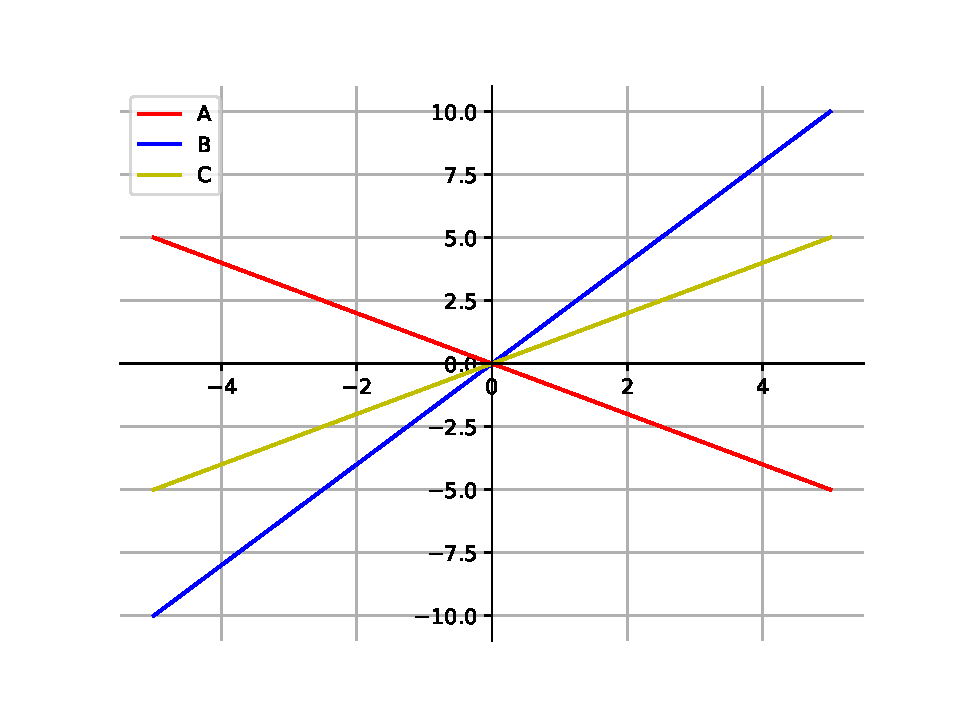
\includegraphics[width=\columnwidth]{./figs/lines/q11a.pdf}
	\caption{Lines of Q.3.7.5}
	\label{fig:qelevena}	
	\end{figure}
	\begin{figure}[!ht]
	\centering
	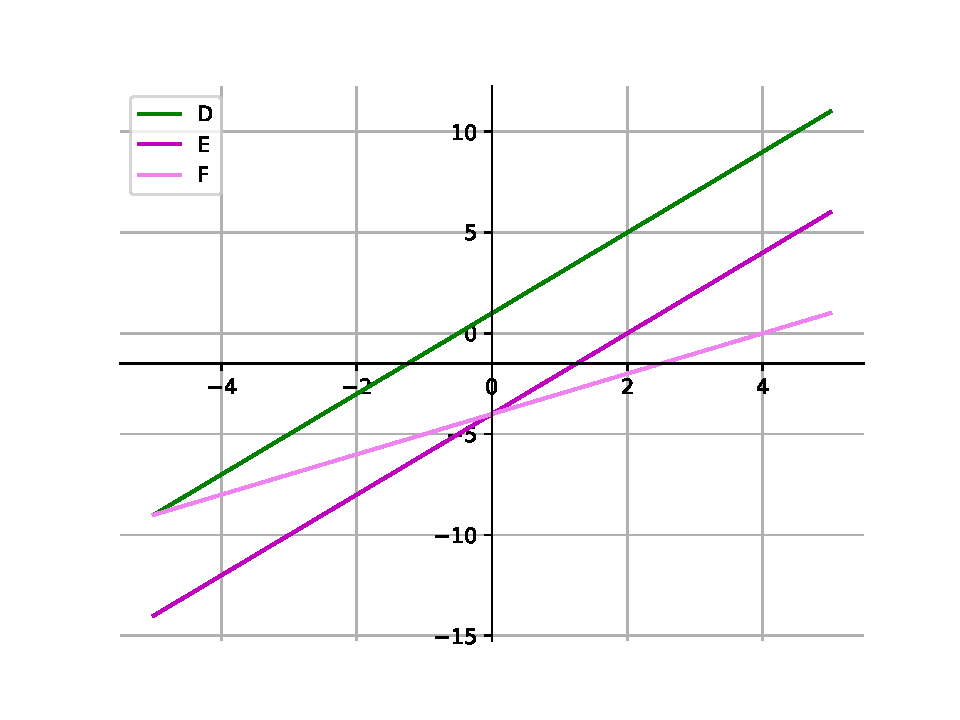
\includegraphics[width=\columnwidth]{./figs/lines/q11b.pdf}
	\caption{Lines of Q.3.7.5}
	\label{fig:qelevenb}	
	\end{figure}
	
\end{enumerate}
